
\begin{multicols}{2}
Une personne observe une éclipse de
Soleil. Cette situation est schématisée par le dessin ci-contre.\\
L'observateur est en $T$ (Terre). Les points $S$ (centre du Soleil),
$L$ (centre de la Lune) et $T$ sont alignés.\\
Le rayon $SO$ du
Soleil mesure 695\,000~km; le rayon $LU$ de la Lune mesure
1\,736~km; la distance $TS$ est 150 millions de km.\\
Calcule
la distance $TL$ (On donnera l'arrondi au km).\\ 
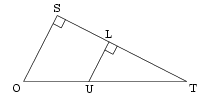
\includegraphics[scale=1]{TR-exo19.png} 
\end{multicols}
